\documentclass{paper}
\usepackage{changepage}
\usepackage{noah}


\usepackage[font=small,labelfont=bf]{caption} 
%% Stuff for inserting code into document
\usepackage{listings}
\usepackage{color}

\definecolor{dkgreen}{rgb}{0,0.6,0}
\definecolor{gray}{rgb}{0.5,0.5,0.5}
\definecolor{mauve}{rgb}{0.58,0,0.82}

\lstset{frame=tb,
  language=Python,
  aboveskip=3mm,
  belowskip=3mm,
  showstringspaces=false,
  columns=flexible,
  basicstyle={\small\ttfamily},
  numbers=none,
  numberstyle=\tiny\color{gray},
  keywordstyle=\color{blue},
  commentstyle=\color{dkgreen},
  stringstyle=\color{mauve},
  breaklines=true,
  breakatwhitespace=true,
  tabsize=3
}

\author{Noah Jeffrey Blair}
\title{Vibrations and Heat Diffusion on the Unit Disc}
\begin{document}
\maketitle
\tableofcontents
\section{Introduction}
Two of the most common partial differential equations that occur in mathematics and physics are the wave equation,
\begin{equation}
\lapl u=\pder{^2 u}{t^2}
\end{equation}
and the heat equation,
\begin{equation}\lapl u=\pder{u}{t}\end{equation}
Both of these equations allow us to analyze the different types of dynamics that occur in PDEs, and also allow us to introduce a method for solving these equations that is applicable for most equations are able to be written into Sturm-Liouville form. We will solve both of these equations on the unit disc $B^2$, with the boundary condition that the function must vanish at the boundary. In the context of the heat equation, this means that we keep the boundary at a fixed temperature. For the wave equation, this means the disc will act like a drumhead, with the ends clamped down. Similar to ODEs, we must also supply initial conditions. Since the heat equation is first order in time, we only need to specify $u(\vect{x},0)$. Since the wave equation is second-order in time, we must specify $u(\vect{x},0)$ and $\der{t}u(\vect{x},0)$.\\
Using physical intuition on heat flow, we assume that the solution will be exponentially decaying in time, and write the solution as:
\begin{equation}u(\vect{x},t)=\psi(\vect{x})\exp(-k^2 t)\end{equation}
Using physical intuition on vibrations, we assume that the solution will be oscillating sinusoidally in time, and write the solution as:
\begin{equation}u(\vect{x},t)=\psi(\vect{x})\exp(i k t)\end{equation}
If we insert both of these into our differential equation, we are left with the following boundary value problem:
\begin{equation}\syst{
    \lapl\psi +k^2\psi=0 \\
    \psi(1,\phi)=0
}\end{equation}
This is known as the Helmoltz equation, and occurs frequently in mathematical physics in the study of waves and heat flow. It can also occur in Quantum Mechanics, describing the Schrodinger Equation for a free particle, the time-independent form of the Black-Scholes equations in economics, and in some simplified equations for fluid dynamics. It comes down to finding the eigenvalues of the Laplace operator on some domain, as well as the eigenfunctions, which in this context are refered to as the normal modes.
\section{The Angular Equation}
Similar to our methods of separating the time component out of the wave and heat equation, we will assume that our normal modes can be written as the product of a function of $r$, and a function of $\phi$. If we insert this ansatz into the Helmholtz equation and rearrange, we obtain:
\begin{equation}
\frac{1}{R(r)}\left[
 r^2\dder{^2 R}{r^2}+r\dder{R}{r}+k^2 r^2
\right]=
\frac{1}{\Phi(\phi)}\dder{^2\Phi}{\phi^2}
\end{equation}
We see that the left-hand side is a function of $r$ only, and the right-hand side is a function of $\phi$ only. Since these two variables are independent of each other, we see that both sides must be equal to a constant. The $\phi$ equation now is:
\begin{equation}\Phi''+C\Phi=0\end{equation}
We also have the implied boundary condition that $\Phi(\phi)$ must be continuous for all $\phi\in S^1$. If $C\leq 0$ then this leads to the trivial solution $\Phi(\phi)=0$ which is unable to match every initial condition. This means that $C>0$. Our solution can therefore be written as:
\begin{equation}\Phi(\phi)=C \exp(i \sqrt{C} \phi)\end{equation}
In order for this function to be continuous, we require that $\sqrt{C}\in\bb{Z}$, and therefore we can write our solution as:
\begin{equation}\Phi(\phi)=c_n e^{i n\phi}\end{equation}
These functions have the useful property that they are orthogonal over one period. We can actually normalize them, to obtain the following two relations:
\begin{equation}f(\phi)=\sum_{n=-\infty}^\infty c_n e^{i n\phi}\end{equation}
\begin{equation}c_n = \frac{1}{2\pi}\int_0^{2\pi} f(\phi) e^{- i n \phi}d\phi\end{equation}
To learn more about this, see the references at the end. The two of these together can be combinend to write the completeness relation:
\begin{equation}\delta(\phi-\phi')=\frac{1}{2\pi}\sum_{n=-\infty}^\infty e^{in(\phi-\phi')}\end{equation}
\section{The Radial Equation}
For our radial equation, we are left with the following differential equation:
\begin{equation}\syst{
    r^2 R''+r R'+(k^2 r^2 - n^2 )R=0 \\
    R(1)=0
}\end{equation}
This is Bessel's differential equation, and has the two linearly independent solutions:
\begin{equation}R(r)=C_1 J_n(kr)+C_2 Y_n(k r)\end{equation}
where the first of these are known as Bessel functions, and the second of these are known as Nuemann functions. The Nuemann functions are infinite at the origin, so we require $C_2=0$. The boundary condition that $R(1)=0$ gives us the condition on $k$:
\begin{equation}J_n(k)=0\end{equation}
Bessel functions have an infinite number of zeros that can be found numerically in programs such as Mathematica. We will let $k=\alpha_{nm}$ to represent the $m$-th zero of the $n$-th Bessel function. In Mathematica, $\alpha_{nm}=\texttt{BesselJZero[n,m]}$.\\
The Bessel functions are also orthogonal on $[0,1]$ and satisfy the following condition:
\begin{equation}\int_0^1 dr J_n(\alpha_{nm} r)J_{n'}(\alpha_{n'm'} r)r=\delta_{nn'}\delta_{mm'}\frac{1}{2}(J_{n+1}(\alpha_{nm}))^2
\end{equation}
We can combine this with the information from the angular solution, to express any function on the unit disc in terms of these eigenfunctions or normal modes.
\begin{equation}
\psi_{nm}(r,\phi)=J_n(\alpha_{nm} r)e^{in\phi}\end{equation}
Using the orthogonality relations, we can express any function in the following way:
\begin{equation}f(r,\phi)=\sum_{m=1}^\infty \sum_{n=-\infty}^\infty  c_{nm}\psi_{nm}(r,\phi)\end{equation}
This is similar to a change of basis in linear algebra. The vector space that we are working with is the set of all functions $f\in L^2(B^2)$ which is to say the set of all functions that are square integrable on the unit ball in two dimensions, or Hilbert space on the unit ball in two dimensions. For a finite dimensional vector space, we can write any vector in terms a given basis for the vector space. For a basis that is orthogonal, we can write any vector and its components using the following:
\begin{equation}\vect{v}=\sum_{i} c_i \vect{e}_i\end{equation} 
\begin{equation}c_i=\frac{(\vect{e}_i,\vect{v})}{(\vect{e}_i,\vect{e}_i)}=\frac{1}{\left|\left| \vect{e}_i\right|\right|^2}(\vect{e}_i,\vect{v})\end{equation}
In order to use this method for our functions, we must define the inner product. Since our complex exponentials are othogonal on $S^1$ and our Bessel functions are orthogonal on $[0,1]$, our functions are orthogonal on the unit disc $[0,1]\times S^1=B^2$. Our inner product is defined as:
\begin{equation}(f,g)=\int_{B^2} f^\star g dA\end{equation}
where the $\star$ denotes complex conjugation. Using this, our expansion coefficients can be written as:
\begin{equation}
    \boxed{
        c_{nm}=\frac{4\pi}{J_{n+1}(\alpha_{nm})^2}\int_0^{2\pi} d\phi \int_0^1 dr f(r,\phi) r e^{-in\phi} J_n(\alpha_{nm}r)
    }
\end{equation}
\section{Physics Behind the Wave Equation}
The wave equation occurs frequently enough in physics and mathematics, that it is important to understand the interpretation of solutions. To start off with, we begin with the wave equation on a fixed interval, which has the interpretation of a wave on a finite string. The motion that we are interested in is transverse motion, so we consider the forces in a direction normal to the line. Newton's second law tells us the following for the dynamics of a small bit of mass on a string:
\begin{equation}
    F_{net}=dm\cdot a=\lambda dx \cdot a
\end{equation}
where $\lambda$ is the linear mass density, and $a$ is the vertical acceleration of the string. If we raise part of the string near this point so that the angle the string makes between these two points is $\theta$, then the force is:
\begin{equation}
    F_{net}=T \sin(\theta + d\theta)-T \sin(\theta)=T\cos(\theta)d\theta)
\end{equation}
where $T$ is the tension in the rope. If we assume small enough displacements, we can approximated $\cos\theta\approx 1$ and write $d\theta= (\partial\theta/\partial x) dx$. Since we are assuming small displacements, we can say that the angle $\theta$ is the slope of the string. We will write the displacement of the string as $u=u(x,t)$, and say that this function must satisfy the following equation:
\begin{equation}\pder{^2 u}{t^2}= \frac{T}{\lambda}\pder{^2 u}{x^2}=\frac{1}{c^2} \pder{^2 u}{t^2}\end{equation}
We are introducing the constant $c$ which is the speed of propogation on the string. This can be absorbed into our time variable, by redifining our unit of time. In higher dimensions, the second partial derivative with respect to position is generalized to the Laplace operator:
\begin{equation}\lapl u=\dive\grad u\end{equation}
This allows us to say that the wave equation in higher dimensions can be written as:
\begin{equation}
    \lapl u=\pder{^2 u}{t^2}
\end{equation}
Harmonic functions (one's that satisfy Laplace's equation $\lapl u=0$) occur whenever the vibrating surface is not accelerating. Therefore, the wave equation describes functions that oscillated about a harmonic function in time. This oscillatory behaviour is the reason for the ansatz that the time dependence is carried by $\exp(i k t)$.
\section{Physics Behind the Heat Equation}
The heat equation, while superficially similar to the wave equation has quite different dynamics, as we will see shortly. The general assumption behind the heat equation is conservation of energy. This conservation law is formlated in terms of a continuity equation:
\begin{equation}\pder{u}{t}+\dive \vect{J}=0\end{equation}
Here $u$ is the energy density, and $\vect{J}$ is the energy flux. This equation states that if energy is flowing into a region, then the energy density must be increasing. In order to find the energy flux, we use Newton's Law of cooling which states that the energy flow is proportional to the temperature difference between two regions. This can be formulated in the following way:
\begin{equation}\vect{J}=-\sigma\grad u\end{equation}
where $\sigma$ is the thermal conductivity. The reason for using the energy gradient instead of the temperature gradient in this equation is that temperature is mearly a useful method for defining the energy. As an example, the equipartition theorem from statistical mechanics tells us that the thermal energy can be written as:
\begin{equation}E=\frac{N f}{2} \cdot k_B T\end{equation}
where $N f$ is the number of degrees of freedom in the system, and $k_B$ is the Boltzmann constant which allows us to convert between temperature and energy. Using this, we may write the heat equation as:
\begin{equation}\pder{u}{t}=\lapl u\end{equation}
Here we have absorbed the thermal conductivity into our definition of time. The interesting part of this equation is that it can be used to describe diffusive processes as well. In fact it can be used to describe many systems that do no violate the first and second law of thermodynamics. The first of these states energy conservation, and the second states that the entropy of a system must increase. This second law is one of the few that does depend on the direction of time. This is why the heat equation is not symmetric in the spatial and temporal variables, when the wave equation is.\\
This system has harmonic solutions whenever the system is not changing in time. Therefore, we see that in time, the solution tends towards a harmonic solution. It is for this reason that solutions to Laplace's equations describe steady state temperature distributions. For the boundary conditions that were used in this system, we have the temperature fixed at the boundary, known as Dirichlet conditions. Physically this means that we have the edges of the disc in an ice bath. This means that our solution tends to one where the temperature is uniform across the disc at zero temperature. This is the reason for the ansatz that the time part of the solution is exponentially decaying in time.
\section{Initial Conditions}
For the heat equation, our general solution can be written as:
\begin{equation}
    u(r,\phi,t)=\sum_{nm} c_{nm}\psi_{nm}(r,\phi)e^{-\alpha_{nm}^2 t}
\end{equation}
To determine the coefficeints $c_{nm}$ we use our initial conditions. When $t=0$, we have:
\begin{equation}u(r,\phi,0)=\sum_{nm}c_{nm}\psi_{nm}\end{equation}
Using our orthogonality relations from before, we see that the coefficeints are given by:
\begin{equation}
    \boxed{
        c_{nm}= \frac{4\pi}{J_{n+1}(\alpha_{nm})^2} \int_{B^2} \psi^\star_{nm} u(r,\phi,0) dA
    }
\end{equation}
If we insert this into our sum, we can define a new function known as the Green's function for this solution:
\begin{equation}G(r,r',\phi,\phi',t)=\sum_{nm}\frac{4\pi}{J_{n+1}(\alpha_{nm})^2} e^{in(\phi-\phi')} J_n(\alpha_{nm} r)J_n(\alpha_{nm}r')e^{-\alpha_{nm} t}\end{equation}
This represents the solution for a distribution whose initial condition is a delta function centered at the origin. Any solution can now be written as:
\begin{equation}u(r,\phi,t)=\int_{B^2} G(r,r',\phi,\phi',t)u(r',\phi',0)dA'\end{equation}
Where the integration is preformed over the primed coordintes.\\
For the wave equation, since the equation is second order in time, we must know the initial displacement of the wave, as well as its initial velocity. To simplify matters, we will rewrite the time component in terms of sine and cosines.
\begin{equation}u(r,\phi,t)=\sum_{nm}\psi_{nm}(r,\phi)\left(a_{nm}\cos(\alpha_{nm} t)+b_{nm}\sin(\alpha_{nm} t)\right)\end{equation}
If we evaluate this at $t=0$, we see that the $a_{nm}$ values are determined by the initial dispacement:
\begin{equation}
    \boxed{
    a_{nm}= \frac{4\pi}{J_{n+1}(\alpha_{nm})^2} \int_{B^2} \psi^\star_{nm} u(r,\phi,0) dA
    }
\end{equation}
If we take the first derivative with respect to time, we see that the $b_{nm}$ coefficients are determined by the initial velocity:
\begin{equation}
    \boxed{
    b_{nm}= \frac{4\pi}{\alpha_{nm}J_{n+1}(\alpha_{nm})^2} \int_{B^2} \psi^\star_{nm} \pder{u}{t}\left.\right|_{t=0} dA
    }
\end{equation}
With this, we now have the solution to both the wave and heat equation for any initial condition.
\section{Dynamics for a Particular Initial Condition}
In principal, the above equations will solve the system for the appropriate initial conditions. As an example of this, consider the following function on the unit disc:
\begin{equation}f(r,\phi)=\frac{9}{4}J_0(\alpha_{03}r)-3 J_1(\alpha_{12}r)\cos(\phi)+\frac{1}{5} J_2(\alpha_{24}r)\sin(2\phi)
\end{equation}
Using Mathematica, we find that the relevant eigenvalues for this problem are, $\alpha_{03}\approx8.6537$, $\alpha_{12}\approx 7.01558$, and $\alpha_{24}\approx 14.7959$. A plot of this function is shown below.\\
\begin{center}
\begin{figure}
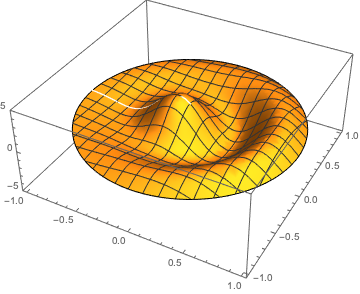
\includegraphics[width = 4.5 cm]{images/initialvalue.png}
\caption{Initial distribution}\end{figure}
\end{center}
\\

If we use this as the initial value of the heat equation, we have the following solution:
\begin{equation}
    u(r,\phi,t)=\frac{9}{4}J_0(\alpha_{03}r)e^{-\alpha_{03}^2 t}-3 J_1(\alpha_{12}r)\cos(\phi)e^{-\alpha_{12}^2 t}+\frac{1}{5} J_2(\alpha_{24}r)\sin(2\phi)e^{-\alpha_{12}^2 t}

\end{equation}
As we can see the components normal modes with larger eigenvalues will decay more quickly which is why the heat equation is so effective at "smoothing" surface. Below are some plots of the solution at later times.

\begin{figure}[!htb]
    \minipage{0.32\textwidth}
      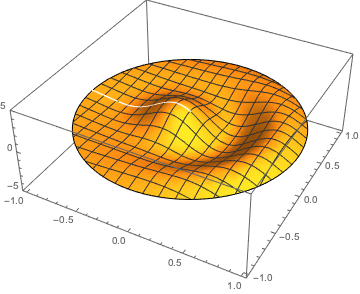
\includegraphics[width=\linewidth]{images/heat1.png}
    \endminipage\hfill
    \minipage{0.32\textwidth}
      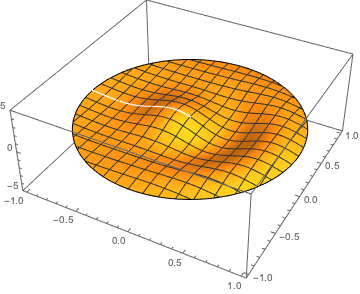
\includegraphics[width=\linewidth]{images/heat2.png}
    \endminipage\hfill
    \minipage{0.32\textwidth}%
      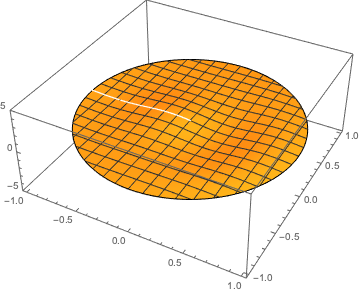
\includegraphics[width=\linewidth]{images/heat3.png}
    \endminipage
    \caption{Solution to the heat equation for various points in time.}
    \end{figure}
If we use this as the initial dislpacement for the wave equation with no initial velocity, we see that the waves interact in interesting ways to produce the following effects.
\begin{equation}
    u(r,\phi,t)=\frac{9}{4}J_0(\alpha_{03}r)\cos(\alpha_{03} t)-3 J_1(\alpha_{12}r)\cos(\phi)\cos(\alpha_{12} t)+\frac{1}{5} J_2(\alpha_{24}r)\sin(2\phi)\cos(\alpha_{12} t)

\end{equation}
We can also use this as the initial distribution for the velocity of the wave. In this case, the displacements are very minor, and we can see that there are only slight deviations from the at rest behaviour.
\begin{figure}[!htb]
    \minipage{0.32\textwidth}
      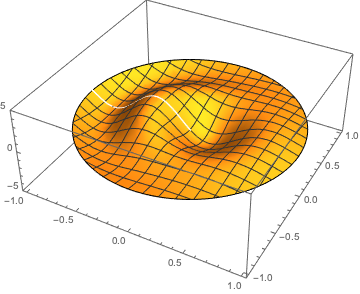
\includegraphics[width=\linewidth]{images/wave1.png}
    \endminipage\hfill
    \minipage{0.32\textwidth}
      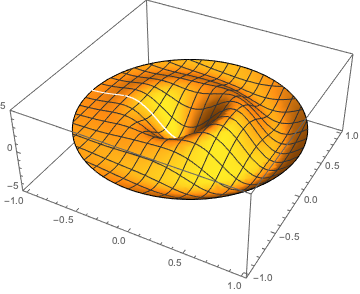
\includegraphics[width=\linewidth]{images/wave2.png}
    \endminipage\hfill
    \minipage{0.32\textwidth}%
      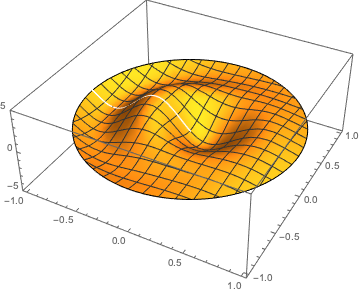
\includegraphics[width=\linewidth]{images/wave3.png}
    \endminipage
    \caption{Solutions to the wave equation for a given initial dispacement.}
    \end{figure}


\begin{equation}
    u(r,\phi,t)=\frac{9}{4 \alpha_{03}}J_0(\alpha_{03}r)\sin(\alpha_{03} t)-\frac{1}{\alpha_{12}} J_1(\alpha_{12}r)\cos(\phi)\sin(\alpha_{12} t)+\frac{1}{5\alpha_{24}} J_2(\alpha_{24}r)\sin(2\phi)\sin(\alpha_{12} t)

\end{equation}

\begin{figure}[!htb]
    \minipage{0.32\textwidth}
      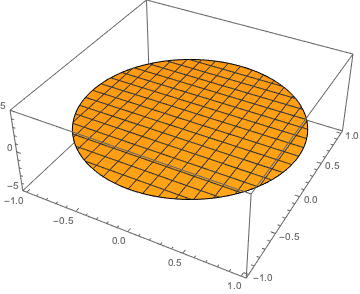
\includegraphics[width=\linewidth]{images/waves1.png}
    \endminipage\hfill
    \minipage{0.32\textwidth}
      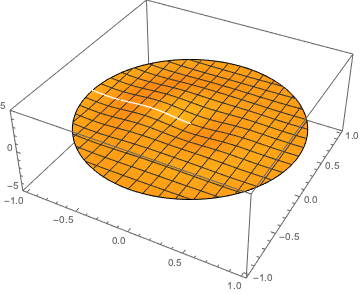
\includegraphics[width=\linewidth]{images/waves2.png}
    \endminipage\hfill
    \minipage{0.32\textwidth}%
      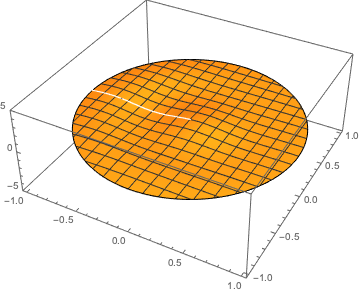
\includegraphics[width=\linewidth]{images/waves3.png}
    \endminipage
    \caption{Solutions to the wave equation for a given initial velocity.}
    \end{figure}
\newpage
\section{Mathematica Code for Animations}
To generate the animations, I use Mathematica's list animate command combined with the three dimensional plot command. The code for this is: \\

\begin{doublespace}
\noindent\(\pmb{\text{DiscAnim}[\text{f$\_$},\{t,\text{t0$\_$},\text{t1$\_$}\},\text{n$\_$}]\text{:=}}\\
\pmb{\text{ListAnimate}[}\\
\pmb{\text{Table}[\text{Plot3D}[f,\{x,-1,1\},\{y,-1,1\},}\\
\pmb{\text{RegionFunction}\to \text{Function}[\{x,y,z\},x{}^{\wedge}2+y{}^{\wedge}2\leq 1],\text{PlotRange}\to \{-5,5\}],}\\
\pmb{\{t,\text{t0},\text{t1},(\text{t1}-\text{t0})/n\}]]}\)
\end{doublespace}
\\
This combined with the various solutions is what allows the animations to be generated. The notebook file for these animations is included with this PDF so that the full dynamics can be appreciated.
\newpage
\section{References}
Asmar, N. H. (2002). \textit{Applied complex analysis with partial differential equations}. New Jersey: Prentice-Hall Inc.\\
\begin{adjustwidth}{2 cm}{}
This book was used to understand differential equations in polar and spherical coordinate systems, as well as certain properties of Bessel functions.\\
\end{adjustwidth}
Farlow, S. J. (2016). \textit{Partial differential equations for scientists and engineers}. New York: Dover Publications, Inc.\\
\begin{adjustwidth}{2 cm}{}
This book was used to understand the basic types of partial differential equations, as well as some methods for solving them in one dimension. It also introduced the physical interpretation of these equations.\\
\end{adjustwidth}
Fetter, A. L., \& Walecka, J. D. (2003). \textit{Theoretical mechanics of particles and continua}. Mineola, NY: Dover Publications. \\
\begin{adjustwidth}{2 cm}{}
This book was used to understand the physical meaning behind the wave and heat equation, as well as some theorems from Sturm-Liouville theory.\\
\end{adjustwidth}
Tolstov, G. P. (2009). \textit{Fourier series}. New York: Dover Publications, Inc.\\
\begin{adjustwidth}{2 cm}{}
This book was used to understand basic properties of Fourier Series and Fourier-Bessel Series, as well as general methods of eigenfunction expansions.
\end{adjustwidth}
\end{document}